\documentclass[final]{beamer}

\usepackage{times}
\usepackage{amsmath,amsthm, amssymb}
\usepackage{wrapfig}
\usepackage[dvipsnames]{tcolorbox}
\usepackage[orientation=landscape,size=a0,scale=1.5]{beamerposter}
\usepackage{tikz}
\usetikzlibrary{shadows.blur} %!!!
\usetikzlibrary{shadows}
\usetheme{gemini}
\usepackage{xcolor}
\usepackage{relsize}


\graphicspath{{./Images/}}

\definecolor{customcolor}{HTML}{D0E0E3}
\definecolor{titlebgcolor}{HTML}{E06666}
\definecolor{myblockcolor}{HTML}{45818E}
\definecolor{blockcolor}{HTML}{FFDADA}%{F9CB9C}

\usecolortheme{whale}
\setbeamercolor{background canvas}{bg=customcolor}
%\setbeamercolor{titlelike}{parent=structure,bg=titlebgcolor}

%\setbeamercolor{titlelike}{parent=structure,bg=cyan}

% If you have N columns, choose \sepwidth and \colwidth such that
% (N+1)*\sepwidth + N*\colwidth = \paperwidth
\newlength{\sepwidth}
\newlength{\colwidth}
\setlength{\sepwidth}{0.025\paperwidth}
\setlength{\colwidth}{0.3\paperwidth}

\newcommand{\separatorcolumn}{\begin{column}{\sepwidth}\end{column}}
\newcommand{\placetextbox}[4]{% \placetextbox{<offset top>}{<offset left/right>}{<align>}{<stuff>}
  \setbox0=\hbox{#4}% Put <stuff> in a box
  \AddToShipoutPictureFG*{% Add <stuff> to current page foreground
    \if#3r
    \put(\LenToUnit{\paperwidth-#1},\LenToUnit{\paperheight-#2}){\vtop{{\null}\makebox[0pt][r]{\begin{tabular}{r}#4\end{tabular}}}}%
    \else
    \put(\LenToUnit{#1},\LenToUnit{\paperheight-#2}){\vtop{{\null}\makebox[0pt][l]{\begin{tabular}{l}#4\end{tabular}}}}%
    \fi
  }%
}%

\newtcolorbox{myblock}[2][]{
  title=\centering\Large\bfseries #2,
  colback=blockcolor,
  colbacktitle=myblockcolor,
  coltitle=white,
  fonttitle=\bfseries,
  colframe=myblockcolor,
  boxrule=0pt,
  toprule=2pt,
  toptitle=5mm,
  bottomtitle=5mm,
  titlerule=0mm,
  arc=5mm,
  outer arc=5mm,
  leftrule=0pt,
  rightrule=0pt,
  bottomrule=0pt,
  boxsep=0pt,
  left=10mm,
  right=10mm,
  top=10mm,
  bottom=10mm,
  shadow={80mm}{-80mm}{90mm}{black!90!white,blur},
  drop shadow=black!90!white,
  enhanced,
}
%   Title ======================================================
% \title{Machines Can Learn Too!}
% \author{H. Fullwood \and S. Hasan \and Y. Wang \and Z. Zhu \and N. An }
% \institute{Target Audience - Elderly Home}

%   Logo ======================================================
\logoleft{
\includegraphics[height=7.5cm]{DUlogo.png}}
% \vspace{8cm}
\logoright{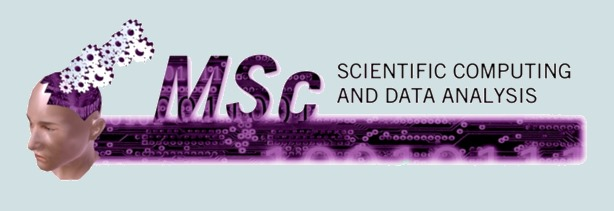
\includegraphics[width=20cm]{MISCADA.jpg}}

%   Body =========================================================
\begin{document}


\begin{frame}{}
\begin{tikzpicture}[remember picture,overlay]
\node [below = 2cm] at (current page.north) [anchor=north,inner sep=0pt] 
  {
    \begin{minipage}{\textwidth}
      \centering
      \begin{tikzpicture}
        \node[rounded corners=10pt, drop shadow, fill=titlebgcolor, text width=0.6\textwidth, minimum height=10cm, align=center, text=white]
        (titlebox) { 
          \bfseries\Huge Machines Can Learn Too! \\[1cm] 
          \normalfont\Large H. Fullwood, S. Hasan, Y. Wang, Z. Zhu, N. An \\ 
          \normalsize Target Audience - Elderly Home 
        };
      \end{tikzpicture}
    \end{minipage}
  };
\end{tikzpicture}
\begin{columns}[t]
\separatorcolumn
\begin{column}{\colwidth}
    \vspace{-2cm}
    \begin{myblock}{How do you think?}
    %\begin{center}
        %What animal is this?
    %\end{center}

    \vspace{-1cm}
    \begin{minipage}{0.49\textwidth}
        \centering
        \begin{figure}
        
\includegraphics[height=1.2\textwidth]{Images/thinking-person.png}
        \end{figure}
    \end{minipage}
    \hfill
    \begin{minipage}{0.49\textwidth}
        \centering
        \begin{figure}
        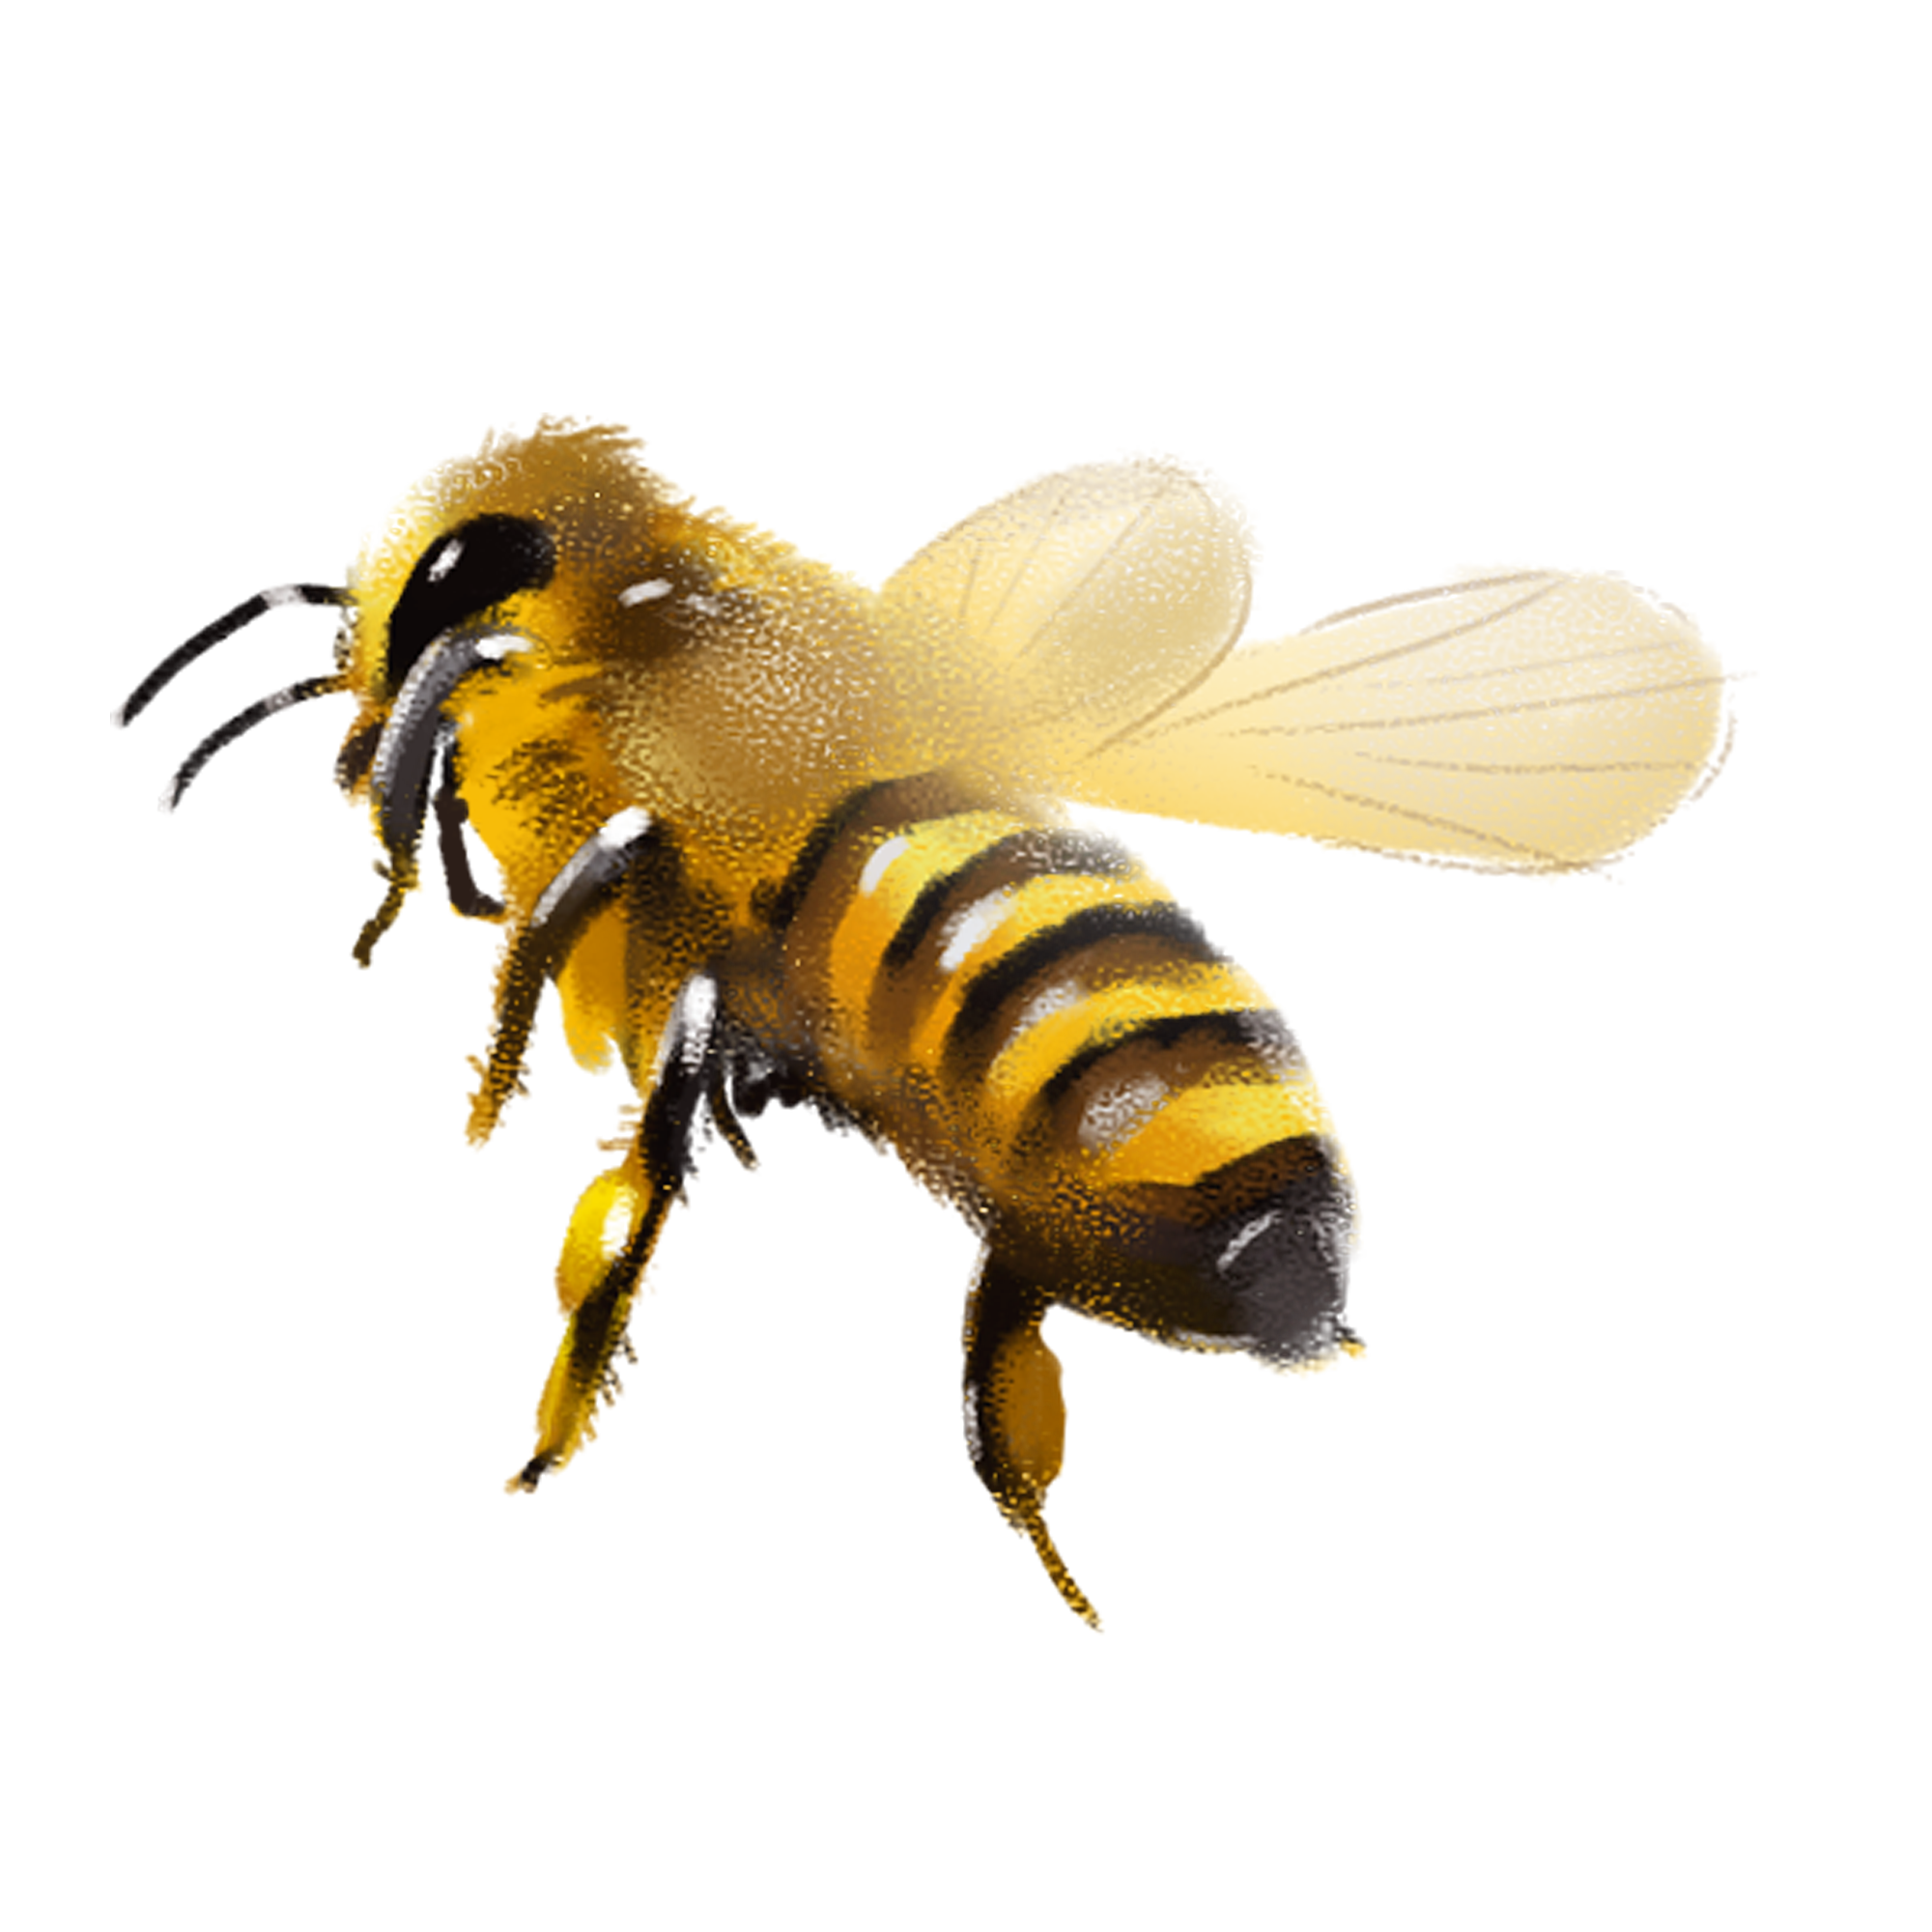
\includegraphics[height=1.0\textwidth]{Bee.png}
        \end{figure}
    \end{minipage}
    
    \vspace{1cm}
    You can probably say “It’s a bee”. You recognise that this is a bee based on your previous experience in seeing bees. An AI machine can also recognize this picture of the bee.
    \end{myblock}

    \begin{myblock}{How do you learn?} 
    You know the image contains a bee because you have seen bees in real life, and you were told that it is a bee. We do the same to teach a machine.
    %\vspace{3cm}
    \raggedright
    \begin{enumerate}
        \item Gather relevant information, e.g.
    \end{enumerate}
    %1. Gather relevant information
    \begin{figure}%{r}{0.4\textwidth}
        \centering
        %\vspace{-6.5cm}
        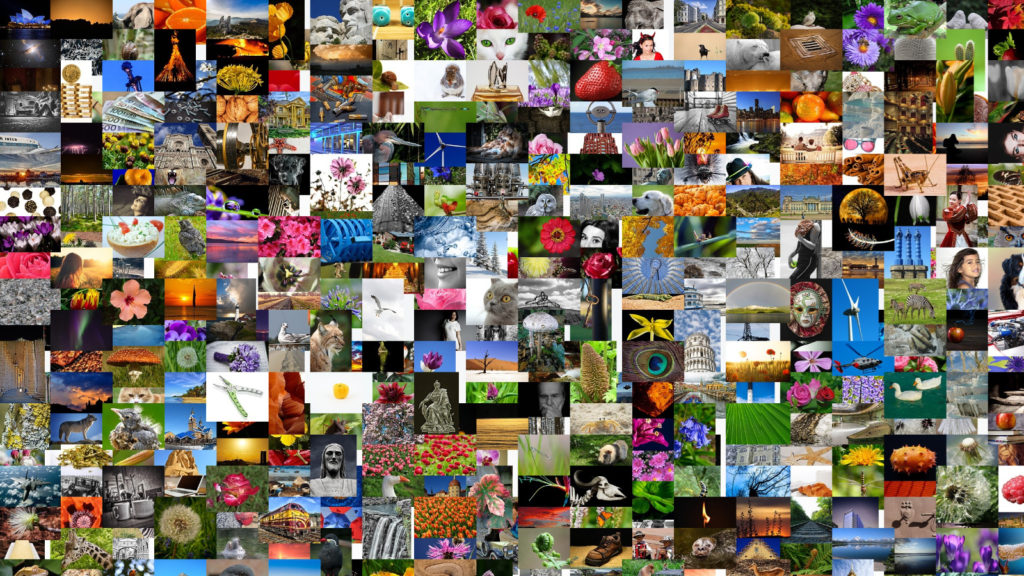
\includegraphics[width=\textwidth]{Images/data.jpg}
    \end{figure}
    \vspace{-0.5cm}
    \begin{enumerate}
        \setcounter{enumi}{1}
        \item Show it to the machine
        \item Write some rules for the machine to analyze and find patterns
        \item Test the machine with new information
    \end{enumerate}
    \end{myblock}
  
\end{column}
    
\separatorcolumn
\begin{column}{\colwidth}
    \vspace{-2cm}
    \begin{myblock}{You can think better!}
    Human thinking is divided into two types:
    \begin{itemize}
      \item \textbf{Fast thinking} - instinct reactions e.g. what is your name?
      \item \textbf{Slow thinking} - slow, effortful and logical e.g. what is your favourite TV show and why?
    \end{itemize}

    \begin{minipage}[t]{0.49\textwidth}
        \smaller[1]
        \begin{tcolorbox}[colback=blockcolor]
        Who is Tom Cruise's mother?
        \end{tcolorbox}
        \vspace{-1cm}
        \begin{tcolorbox}[colback=blockcolor]
        Tom Cruise's mother is Mary Lee Pfeiffer [...]
        \end{tcolorbox}
    \end{minipage}
    \hfill%
    \begin{minipage}[t]{0.49\textwidth}
        \smaller[1]
        \begin{tcolorbox}[colback=blockcolor]
        Who is Mary Lee Pfeiffer's son?
        \end{tcolorbox}
        \vspace{-1cm}
        \begin{tcolorbox}[colback=blockcolor]
        As of [...] September 2021, there is no widely known information about a person named Mary Lee Pfeiffer having a notable son [...]
        \end{tcolorbox}
    \end{minipage}
    
    \vspace{0.7cm}
    AI is good at fast thinking, but bad at logical thinking. They don't have emotion or rational thought and do not actually understand that a bee is a bee.
    Many AI models are only good at one task, the one that tells you that an image contains a bee, can’t explain the surroundings of the bee in the image (unless specifically taught to do so).
    \end{myblock}

    \begin{myblock}{Where do they shine?}
    \begin{minipage}[t]{0.49\textwidth}
        \begin{center}
            \underline{Image Generation}
        \end{center}
        \begin{tcolorbox}[colback=blockcolor]
            Delicious burger painted in the style of a starry night.
        \end{tcolorbox}
        \vspace{-1.1cm}
        \begin{tcolorbox}[colback=blockcolor]
        \begin{figure}
            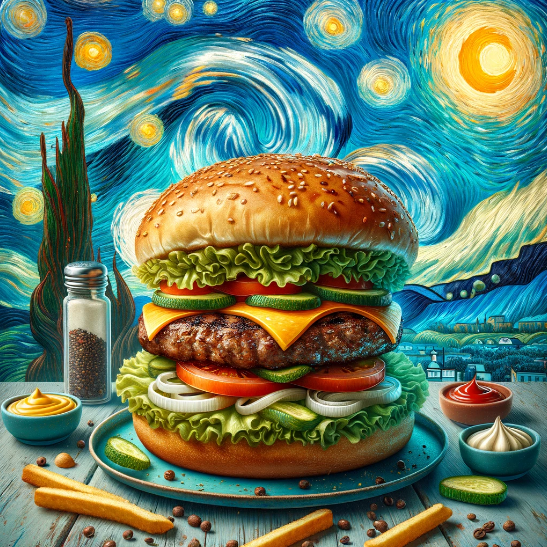
\includegraphics[width=\textwidth,height=0.8\textwidth]{Images/Burger.png}
        \end{figure}
        \end{tcolorbox}
    \end{minipage}
    \hfill%
    \begin{minipage}[t]{0.49\textwidth}
        \begin{center}
            \underline{Recommendations}
        \end{center}
        \begin{tcolorbox}[colback=blockcolor]
            What can I make with eggs, flour and milk?
        \end{tcolorbox}
        \vspace{-1.1cm}
        \begin{tcolorbox}[colback=blockcolor]
        \begin{enumerate}
            \item Pancakes
            \item Crepes
            \item Yorkshire Pudding
            \item Waffles
            \item Quiche Base
            \item Dutch Baby Pancake
            \item Popover
        \end{enumerate}
        \end{tcolorbox}
    \end{minipage}
    
    %\begin{figure}
    %    \centering
    %    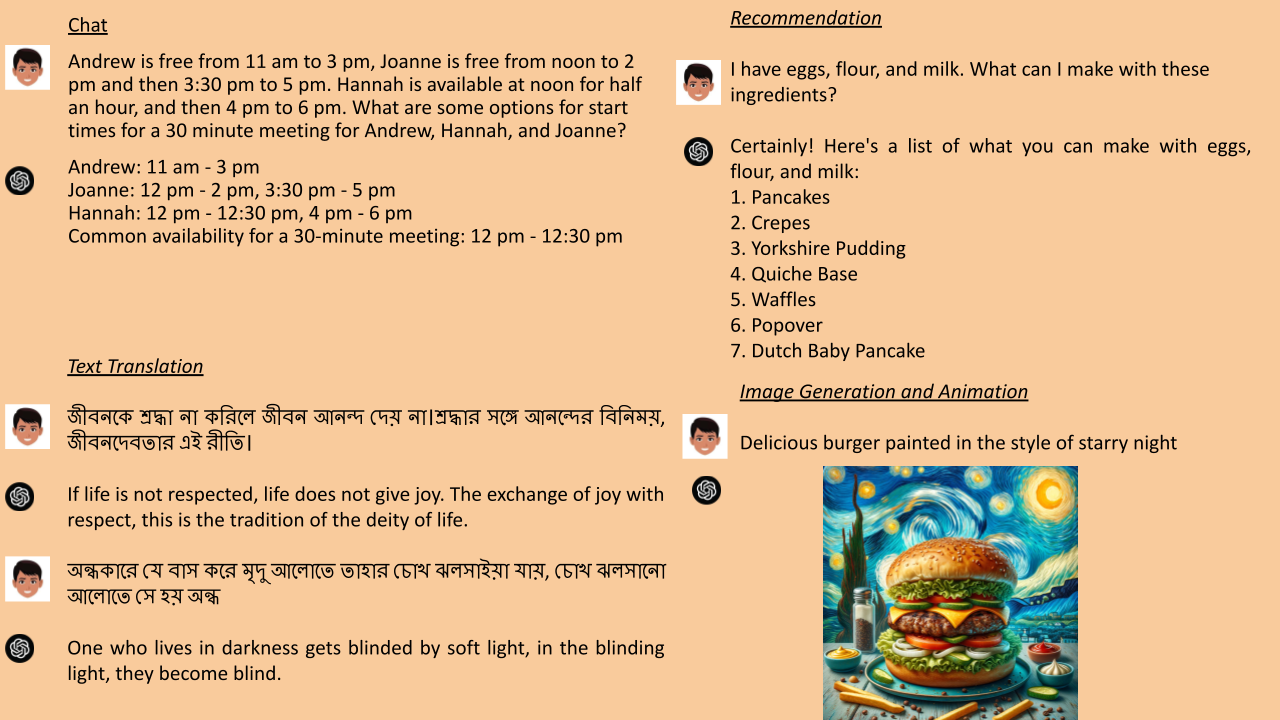
\includegraphics[width=1.0\textwidth]{Images/shine.png}
        % \caption{The Wednesday Adans}
        % \label{fig: The Wednesday Adans}
    %\end{figure}
 
    \end{myblock}

    \begin{myblock}{How is it used?}
    \begin{itemize}
        \item \textbf{Chat companion} - ChatGPT, Gemini, LLaMA, Alexa
        \item \textbf{Generating images} - DALL-E, Stable Diffusion
        \item \textbf{Organizing things and cleaning} - Atlas, Optimus, Roomba
        \item \textbf{Self-driving car} - Tesla Autopilot
        \item \textbf{Health Monitoring} - Smart Watch
        % \item  \textbf{Robotics} - Atlas, Spot, Optimus
    \end{itemize}
    
    \end{myblock}
    
\end{column}

\separatorcolumn
\begin{column}{\colwidth}
    \vspace{-2cm}
    \begin{myblock}{Try it yourself! (Demo)}
    \begin{wrapfigure}[1]{r}{0.28\textwidth}
        \vspace{-5cm}
        
\includegraphics[width=0.28\textwidth]{Images/QR.png}
    \end{wrapfigure}

    \begin{minipage}{0.7\textwidth}
        \begin{enumerate}
            \item Go to the following link or use the QR code: https://neural-style-transfer-app.ew.r.appspot.com/
            \item Agree to the terms and conditions
            \item Upload your photo by clicking "Upload image"
        \end{enumerate}
    \end{minipage}
    \begin{enumerate}
            \setcounter{enumi}{4}
            \item Upload your style by clicking "Upload your own Style" or Select one from the website
            \item Click "Transfer Style" - the AI model will generate your first image in the style of the 
            second image.
    \end{enumerate}
    
    \vspace{1.5cm}
    \begin{figure}
      \centering
        \begin{minipage}{.5\textwidth}
            \centering
            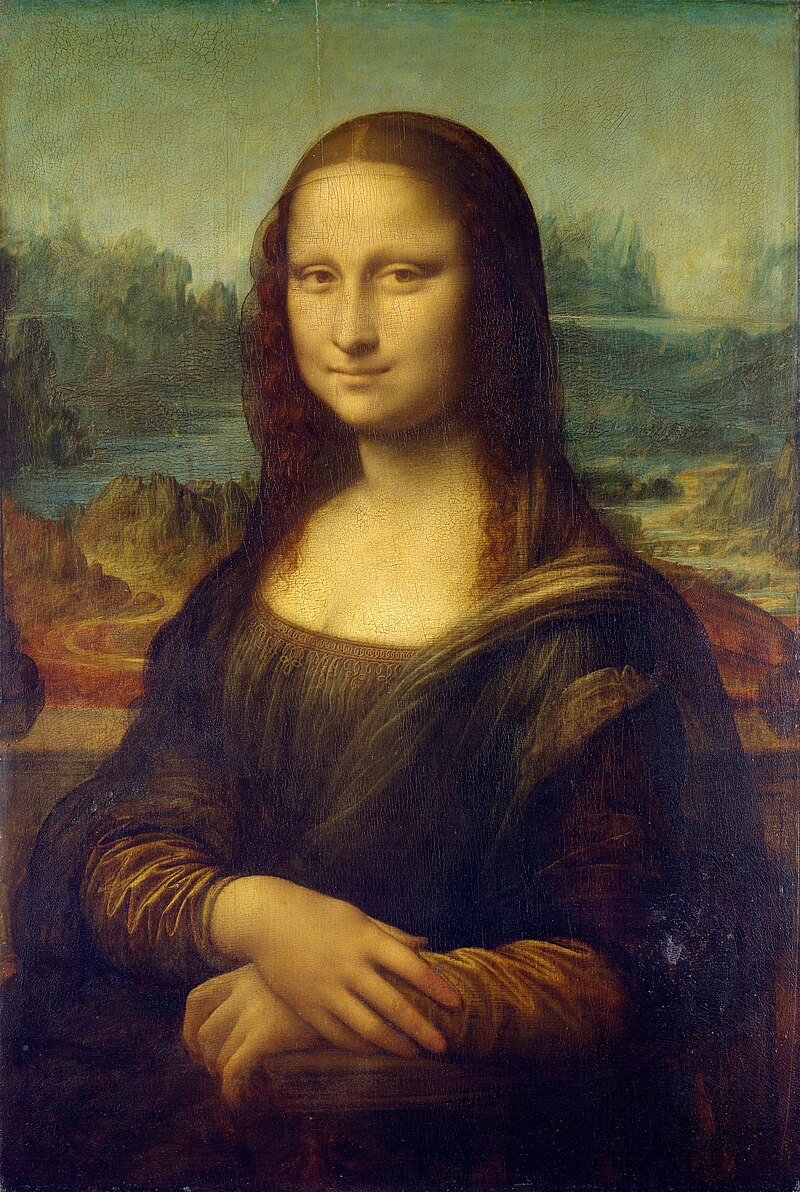
\includegraphics[width=.7\linewidth]{Images/Mona_Lisa.jpg}
            
            Mona Lisa
        \end{minipage}%
        \begin{minipage}{.5\textwidth}
            \centering
            \vspace{4.0cm}
            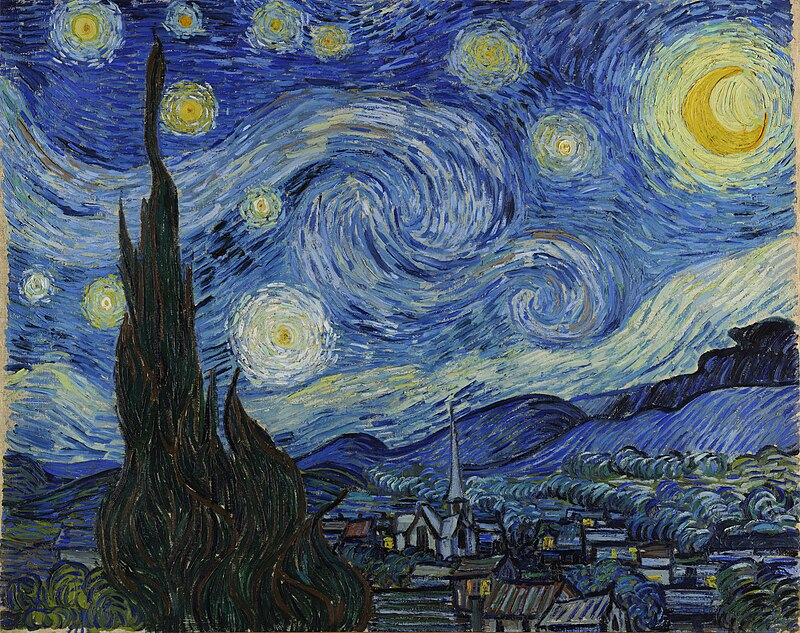
\includegraphics[width=1.0\linewidth]{Images/Starry_Night.jpg}
            
            The Starry Night
        \end{minipage}
      % \caption{Example of a figure side by side.}
    \end{figure}
    \vspace{1cm}
    \begin{figure}
        \centering
        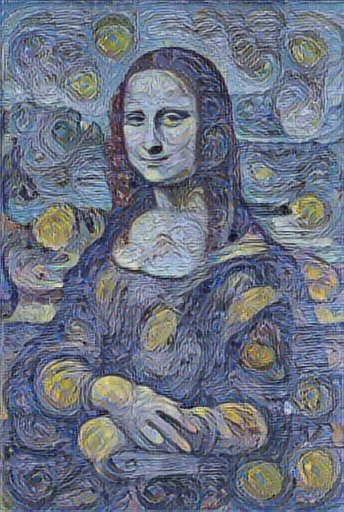
\includegraphics[width=0.4\textwidth]{Images/Style-Transfer.jpg}
        
        Mona Lisa with the artistic style of The Starry Night
    \end{figure}
    \vspace{1.5cm}
    \end{myblock}
\end{column}


\end{columns}
\end{frame}
\end{document}
%    \vfill
%    \begin{block}{\large Fontsizes}
%      \centering
%      {\tiny tiny}\par
%      {\scriptsize scriptsize}\par
%      {\footnotesize footnotesize}\par
%      {\normalsize normalsize}\par
%      ...
%    \end{block}
%    
%    \vfill
%    \begin{columns}[t]
%      \begin{column}{.30\linewidth}
%        \begin{block}{Introduction}
%          \begin{itemize}
%%          \item some items
%          \item some items
%%          ...
 %         \end{itemize}
 %       \end{block}
 %     \end{column}
 %     \begin{column}{.48\linewidth}
 %       \begin{block}{Introduction}
 %         \begin{itemize}
 %         \item some items and $\alpha=\gamma, \sum_{i}$
 %         ...
 %         \end{itemize}
 %         $$\alpha=\gamma, \sum_{i}$$
 %       \end{block}
  %      ...

%      \end{column}
%    \end{columns}
%  \end{frame}
